\pagebreak
\section{Qualità}
La qualità perseguita nel presente documento si basa sugli standard ISO/IEC 15504  e ISO/IEC 9126 con l'obiettivo di approfondirne incrementalmente la copertura. Tutti i processi seguono il metodo \glossario{PDCA} che prevede l'iterazione ripetuta tra i quattro stadi, incrementando di volta in volta quanto prodotto. La struttura di qualifica assicura un incremento della qualità ad ogni ciclo. \\
	\begin{figure}[h]
	\centering 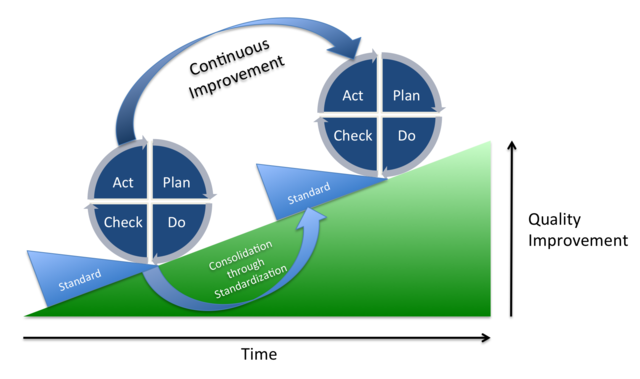
\includegraphics[width=1\textwidth]{PDCA.png}
	\caption{Continuous quality improvement with PDCA}
	\end{figure}
	
	\begin{enumerate}
		\item \textbf{PLAN}: vengono stabiliti gli obiettivi e i processi necessari per raggiungere i risultati attesi;
		\item \textbf{DO}: viene implementato il punto precedente, creando una parte del prodotto. In questo stadio vanno misurate le metriche;
		\item \textbf{CHECK}: vengono studiate ed elaborate le metriche rilevate al punto precedente, un confronto con i risultati attesi sarà il riscontro se quanto operato va nella direzione giusta. Vanno considerate metriche come la \emph{Schedule Variance} (vedi \ref{ScheduleVariance}) e la completezza dei risultati attesi soddisfatti, vanno elaborati grafici e tabelle per avere una visione chiara di quanto rilevato;
		\item \textbf{ACT}: vengono svolte le azioni correttive emerse dall'analisi del punto precedente e tutti i membri del gruppo vengono informati. Si potrà eseguire tramite riunioni o strumenti di messaggistica interna al gruppo. Terminato questo stadio si procederà con una nuova iterazione a partire dal punto 1.
	\end{enumerate}

	\subsection{Qualità dei processi}
	Definita in ISO/IEC 15504 come \glossario{SPICE}, specifica come la qualità è collegata alla maturazione dei processi. Vengono individuati dei livelli di maturità al quale il fornitore può fare riferimento per determinare le proprie capacità organizzative. Vengono definiti:
	\begin{itemize}
		\item Dei \textbf{Modelli di riferimento} su:
			\begin{itemize}
				\item \emph{dimensione del processo};
				\item \emph{livelli di capacità dei processi}:
					\begin{etaremune}
						\item ottimizzato
						\item predicibile
						\item stabilito
						\item gestito
						\item eseguito
						\item incompleto
					\end{etaremune}
					La capacità di un processo viene misurata tramite degli attributi che sono assimilabili alle metriche dei processi individuate in \ref{MetricheProcessi}, in particolare la \emph{Schedule Variance} permette di capire se un processo è incompleto o gestito; il gruppo giungerà a maturazione quando i processi diventeranno predicibili ossia quando la \emph{Schedule Variance} subirà al più lievi oscillazioni;
			\end{itemize}
		\item Delle \textbf{Stime} che si concretizzano in una struttura per la misurazione composta da:
			\begin{itemize}
				\item I \emph{processi} di misurazione, indicati nel \PianoDiProgetto ;
				\item Un \emph{modello} per la misurazione identificabile in questo documento;
				\item Gli \emph{strumenti} utilizzati, specificati nelle \NormeDiProgetto .
			\end{itemize}
		\item Le \textbf{Competenze e Qualifiche} di chi controlla; lo standard redige in modo rigoroso una serie di attività volte a formare chi opera l'attività di stesura del \emph{Piano di Qualifica} e \emph{Verifica}. Tali competenze sono assenti all'interno del gruppo e, considerato che effettuare una formazione in linea con quanto specificato dallo standard sarebbe impossibile, tutti i membri si impegnano a studiare ed applicare al meglio quanto descritto in questo documento.
	\end{itemize}
	
	\subsection{Qualità del prodotto software}
	Specificata in ISO/IEC 9126 si suddivide in:
	\begin{itemize}
		\item \textbf{Quality model}: classifica la qualità del software in un set di caratteristiche che verranno approfondite nel corso del progetto:
			\begin{itemize}
				\item Functionality;
				\item Reliability;
				\item Usability;
				\item Efficiency;
				\item Maintainability;
				\item Portability.
			\end{itemize}
			Allo stato attuale, il gruppo non è in grado individuare un modello specifico per lo \glossario{stack} tecnologico da utilizzare.
		\item \textbf{External metrics}: sono le metriche rilevate tramite analisi dinamica, verranno specificate con il concretizzarsi della \emph{Specifica Tecnica};
		\item \textbf{Internal metrics}: sono le metriche rilevate in analisi statica specificate in \ref{MisureMetriche};
		\item \textbf{Quality in use metrics}: si tratta di metriche rilevabili allo stato di prodotto \emph{usabile} in condizioni reali, si rimanda la definizione di tale aspetto a quando verranno trattate le considerazioni sull'usabilità del prodotto in uno scenario di utilizzo reale, questo deve avvenire non oltre la \emph{Progettazione di Dettaglio e Codifica}.
	\end{itemize}

